\begin{abwframe}
\node[anchor=north west,inner sep=0pt,outer sep=0pt] at (40.625,-55.791) {\begin{minipage}[t][69.584bp][c]{878.75bp}\setlength{\parindent}{0pt}\setlength{\parskip}{0pt}{\TimesNR\fontsize{44}{49.28}\selectfont\color{cBC0031}\bfseries\raggedright Universal Approximation Theorem\par}\end{minipage}};
\node[anchor=north west,inner sep=0pt,outer sep=0pt] at (40.625,-158.857) {\begin{minipage}[t][299.652bp][c]{744.358bp}\setlength{\parindent}{0pt}\setlength{\parskip}{0pt}{\TimesNR\fontsize{24}{26.88}\selectfont\color{c000000}\raggedright “A feedforward network with a single hidden layer is sufficient to represent any function”\par}\end{minipage}};
\node[anchor=north west,inner sep=0pt,outer sep=0pt] at (179.593,-189.577) {\begin{minipage}[t][77.62bp][t]{600.723bp}\setlength{\parindent}{0pt}\setlength{\parskip}{0pt}{\TimesNR\fontsize{32}{35.84}\selectfont\color{c000000}\raggedright “\ldots{} but the layer may be infeasibly large and may fail to learn and generalize correctly.”\par}\end{minipage}};
\node[anchor=north west,inner sep=0pt,outer sep=0pt] at (753.686,-397.427) {\begin{minipage}[t][38.845bp][t]{600.723bp}\setlength{\parindent}{0pt}\setlength{\parskip}{0pt}{\TimesNR\fontsize{32}{35.84}\selectfont\color{c751B68}\raggedright Ian Goodfellow\par}\end{minipage}};
\node[anchor=north west,inner sep=0pt,outer sep=0pt] at (784.983,-192.678) {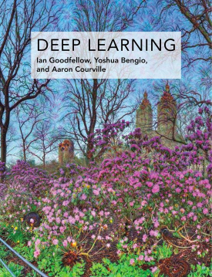
\includegraphics[width=159.216bp,height=207.85bp]{assets/source/slide-47-object-005.png}};
\node[anchor=north west,inner sep=0pt,outer sep=0pt] at (56.693,-499.702) {\begin{minipage}[t][11.952bp][c]{324bp}\setlength{\parindent}{0pt}\setlength{\parskip}{0pt}{\TimesNR\fontsize{10}{11.2}\selectfont\color{c7F7F7F}\raggedright Analytics for a Better World Lecture 2\par}\end{minipage}};
\node[anchor=north west,inner sep=0pt,outer sep=0pt] at (880.898,-499.702) {\begin{minipage}[t][11.952bp][c]{22.409bp}\setlength{\parindent}{0pt}\setlength{\parskip}{0pt}{\TimesNR\fontsize{10}{11.2}\selectfont\color{c7F7F7F}\bfseries\raggedleft 47\par}\end{minipage}};
\end{abwframe}
